\documentclass[lettersize,journal]{IEEEtran}
\usepackage{amsmath,amsfonts}
\usepackage{algorithmic}
\usepackage{algorithm}
\usepackage{array}
\usepackage[caption=false,font=normalsize,labelfont=sf,textfont=sf]{subfig}
\usepackage{textcomp}
\usepackage{stfloats}
\usepackage{url}
\usepackage{verbatim}
\usepackage{graphicx}
\usepackage[backend=bibtex]{biblatex}
\usepackage[utf8]{inputenc}
%\usepackage{tikz}
\usepackage{pgfplots}

\pgfplotsset{width=4cm,compat=newest}

% Externalize PGF figures
\usepgfplotslibrary{external}
\tikzexternalize


%\DeclareUnicodeCharacter{2212}{−}
%\usepgfplotslibrary{groupplots,dateplot}
%\usetikzlibrary{patterns,shapes.arrows}
%\pgfplotsset{compat=newest}tikztikz

\addbibresource{ref.bib}
\graphicspath{{./images/}}

\begin{document}
	
    \title{COMSOL Simulation of a Dual-axis MEMS Accelerometer with T-shape Beams}

    \author{Leonardo Bove\\
            \textit{Dipartimento di Ingegneria dell'Informazione}\\
            \textit{University of Pisa}\\
            \texttt{l.bove3@studenti.unipi.it}}

    \maketitle
	
    \begin{abstract}
        This paper presents the mechanical response of a MEMS dual-axis accelerometer with T-shaped beams for different values of X and Y axes accelerations. The original design idea and simulation are taken from an excerpt from the \textit{Proceedings of the 2015 COMSOL} Conference in Boston \cite{original}. The aim of this paper is to validate the results obtained in the reference through a COMSOL 6.0 Multiphysics simulation. The results show the inertial mass displacement and the induced stress. Beams equivalent elastic constants and displacement sensitivities to accelerations (\(S_{dx}\), \(S_{dy}\)) along X and Y axes were evaluated and compared to theoretical forecasts. Accelerations up to 50g were simulated. Moreover, the dependence of the  sensitivity along the X axis was evaluated for different values of the spring arms' dimensions \(w_{bx}\) and \(t_{bx}\). The obtained results are compared with the theoretical models proposed in the referenced paper.
    \end{abstract}
	
    \section{Introduction}
        \IEEEPARstart{N}{}owadays, MEMS accelerometers have an extensive applications range: consumer electronics, automotive systems, aerospace, and robotics. Small size, together with low power consumption and cost-effectiveness, turn them into the basis in inertial navigation and motion sensing. One critical evolution in the technology for MEMS accelerometers involves the development of dual-axis devices that can measure accelerations along two orthogonal axes in a single package. These designs improve integration efficiency and reduce the complexity of aligning several single-axis accelerometers.
        
        This report focuses on the analysis and optimization of a MEMS dual-axis accelerometer featuring T-shaped beams. The special geometry of these beams allows for the measurement of accelerations along both the X and Y axes through differential capacitance sensing. Theoretical basics of the accelerometer design, as mentioned in the referred article, are modeled and simulated in COMSOL Multiphysics.
        
        The main objectives of this study are:
        \begin{itemize}
        \item Calculating the displacement of the inertial mass and the induced stress for several acceleration inputs along both the X and Y axes. The range of accelerations is the same as the one simulated in the original paper, i.e. up to 50g in both directions.
        \item Obtaining the equivalent elastic constants of the beams and the device displacement sensitivity to accelerations, \(S_{dx}\) and \(S_{dy}\), in both axes.
        \item Carrying out a parametric analysis to study the dependence of sensitivity, \(S_{dx}\), on the spring arm dimensions \(w_{bx}\) and \(t_{bx}\).
        \item Comparing simulation results with theoretical predictions in order to validate the model and identify areas for possible design improvements.
        \end{itemize}
        
    \section{Structure Design and Analysis}
        The structure of the analysed device is shown in figure \ref{fig:dev-struct}. This accelerometer is designed to be fabricated with polysilcon surface-micromachining. The whole device is symmetric vertically and horizontally: these symmetries will be exploited later to reduce the COMSOL model size.
        
        The central movable mass is anchored through two T-shape beams. Each T-shape beam consists of one straight beam and two folded beams.
        
        Attached to the central mass, there are 64 movable fingers, divided into 8 groups. Each side of the central mass has 2 groups of fingers. Each of them faces one fixed finger and the capacitance between those is used to sense the external acceleration. The vertical fingers (aligned along the Y axis) together with the straight beams are used to sense acceleration along X direction, so they are called X-beams and X-capacitance groups. On the other hand, the horizontal fingers (aligned along the X axis) together with the folded beams are used to sense acceleration along Y direction, so they are called Y-beams and Y-capacitance groups. Due to the symmetry of the device, two of the four groups of X movable fingers have fixed fingers on the left side, whereas the other two groups have them on the right. Similarly, this apply to Y-movable fingers groups: two of them have fixed fingers in the upper side, the other two on the down side. This is helpful for obtaining a differential capacitance, as will be explained in \ref{sssec:capacity}.
        
        %\includegraphics{full_dev}
        
        \begin{figure}[h!]
            \centering
            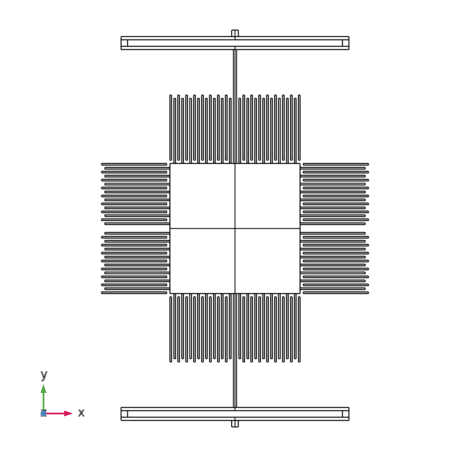
\includegraphics[width=1.0\linewidth]{full_device_geometry.png}
            \caption{Device structure.}
            \label{fig:dev-struct}
        \end{figure}
        
        \subsection{Device Geometrical Sizing}
        A detailed view of the geometrical model used in this COMSOL simulation is presented in figure \ref{fig:dev_quotes}. As anticipated, in order to reduce the size of the model, only \(\frac{1}{8}\) of the whole device was simulated, taking advantage of the symmetries along X, Y and Z axes.
        
        \begin{figure}[h!]
            \centering
            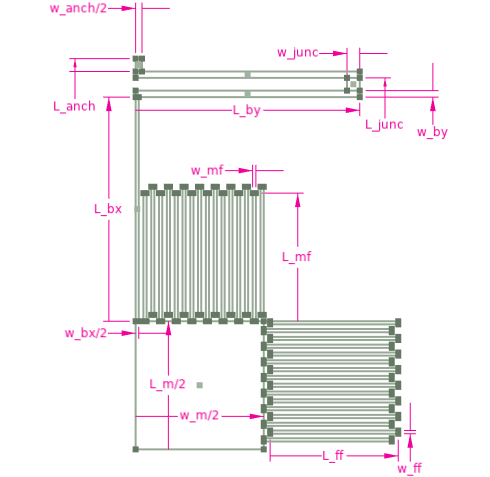
\includegraphics[width=1.0\linewidth]{device_size.png}
            \caption{Device dimensions.}
            \label{fig:dev_quotes}
        \end{figure}
        
        Table \ref{tab:size} shows all the geometrical parameters of the device, which are identical to those used in \cite{original}. The only dimensions that were missing are those of the folded beams junction element.
        
        \begin{table}[h!]
            \centering
            \caption{Device components dimensions}
            \label{tab:size}
            \begin{tabular}{|c|c|c|c|}
                \hline
                \textbf{Components}   & \textbf{Quantity} & \textbf{Length (\(\mu m\))} & \textbf{Width (\(\mu m\))} \\ \hline
                Central mass          & 1                 & 800                  & 800                 \\ \hline
                Movable fingers       & 64                & 400                  & 10                  \\ \hline
                Fixed fingers         & 64                & 400                  & 10                  \\ \hline
                Folded beam segments  & 8                 & 700                  & 20                  \\ \hline
                Folded beam junctions & 4                 & 40                   & 40                  \\ \hline
                Straight beams        & 2                 & 700                  & 20                  \\ \hline
                Anchors               & 2                 & 40                   & 40                  \\ \hline
            \end{tabular}
        \end{table}
        
        The whole geometrical description of the device was parametrized on COMSOL, in order to make it more flexible and allow for geometrical parametric sweeps. The parameters labels used, as shown in figure \ref{fig:dev_quotes}, are the following:
        
        \begin{itemize}
            \item \(L_m, w_m, t_m\): length, width and thickness of the central mass.
            \item \(L_{bx}, w_{bx}, t_{bx}\): length, width and thickness of the straight X beam.
            \item \(L_{by}, w_{by}, t_{by}\): length, width and thickness of the folded Y beams segments.
            \item \(L_{junc}, w_{junc}\): length and width of the folded Y beams junctions. The thickness is the same as the other segments.
            \item \(L_{anch}, w_{anch}\): length and width of the anchor. The thickness is the same as the folded beams.
            \item \(L_{mf}, w_{mf}, t_{mf}\): length, width and thickness of the movable fingers.
            \item \(L_{ff}, w_{ff}\): length and width of the fixed fingers. The thickness is the same as the movable fingers.
        \end{itemize}
        
        The 8 fixed fingers at the vertices of the central mass are assumed to be aligned with the side of the mass itself, as shown in figure \ref{fig:ff-detail}.
        
        \begin{figure}
            \centering
            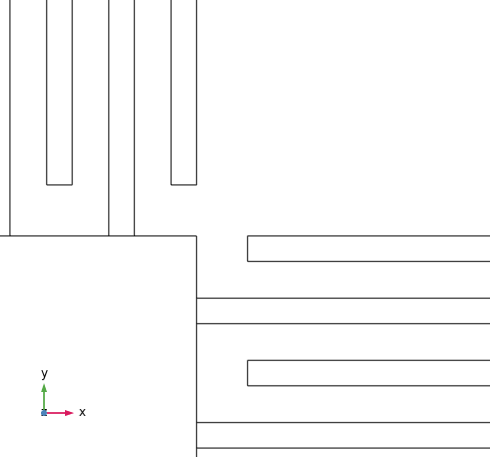
\includegraphics[width=1.0\linewidth]{device_ff_detail.png}
            \caption{Fixed fingers alignment detail.}
            \label{fig:ff-detail}
        \end{figure}
        
        The fingers of each group are assumed to be equally spaced and this spacing is the same for both the vertical and the horizontal groups. This spacing is parametrically defined from the available space for the movable fingers in the upper mass side, where the width of the straight beam must be taken into account. This distance between each movable and fixed fingers \(d\) is defined as follows:
        
        \begin{equation}
            d = \frac{\frac{L_m}{2}-8*(w_{mf}+w_{ff})-\frac{w_{bx}}{2}}{16}
        \end{equation}
        
        Also the overlapping between the movable and fixed fingers had to be assumed and it was parametrically defined for both the vertical (\(L_{ov,v}\)) and horizontal (\(L_{ov,h}\)) fingers and set to \(L_{ov,v}=L_{ov,h}=380\mu m\).
        
        The outer air box that contains the device was defined to be larger than the maximum dimensions of the accelerometer by an offset of \(box_{offset}=50\mu m\). This is true for every side of the accelerometer, except for the three symmetry planes.
        
        \subsection{Theoretical Analysis}
        We now discuss the mathematical models used to predict the behaviour of this system.
        
        \subsubsection{Beams Stiffness}
        The simplified mechanical model of the system is the following:
        
        
        \subsubsection{Displacement Sensitivity To Accelerations}
        \subsubsection{Capacitance Sensing}\label{sssec:capacity}
        As anticipated before, thanks to the mirrored position of the fixed fingers relative to the movable fingers (e.g. in the upper-right side fixed fingers are on the right of their movable fingers, whereas in the upper-left side the opposite happens) differential capacitance can be measured to sense the displacement of the mass due to inertial force.
        
    
    \section{COMSOL Multiphysics}
    \begin{figure*}[!ht]
        \centering
        \subfloat[]{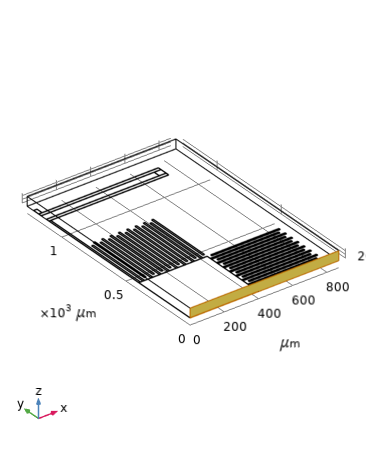
\includegraphics[width=0.3\textwidth]{y_symmetry_plane.png}%
            \label{fig:y-plane}}
        \hfil
        \subfloat[]{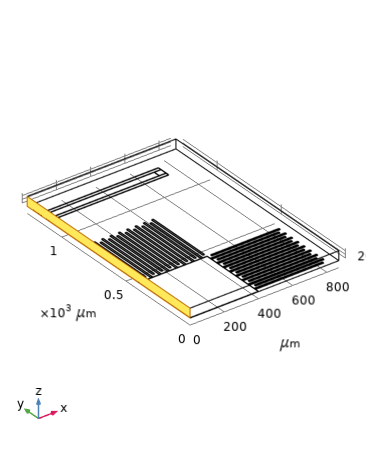
\includegraphics[width=0.3\textwidth]{x_symmetry_plane.png}%
            \label{fig:x-plane}}
        \hfil
        \subfloat[]{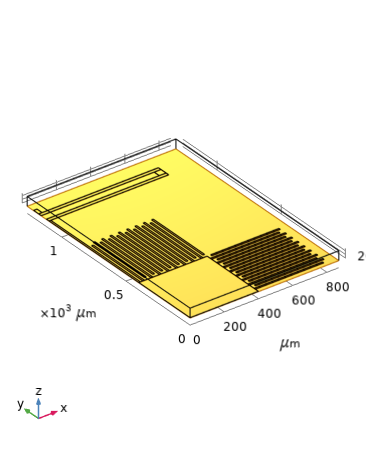
\includegraphics[width=0.3\textwidth]{z_symmetry_plane.png}%
            \label{fig:z-plane}}
        \caption{Symmetry planes, (a) \(y=0\), (b) \(x=0\) and (c) \(z=0\).}
        \label{fig:symmetry-planes}
    \end{figure*}
    \subsection{Simulation Setup}
        The COMSOL modules used for the simulation of the analysed system are:
        \begin{itemize}
            \item \textit{Solid Mechanics}
            \item \textit{Electrostatics}
            \item \textit{Electromechanics}        
        \end{itemize}
        Following \cite{original}, the used materials are:
        
        \begin{itemize}
            \item Air (Built-in)
            \item Polycrystalline silicon (MEMS)
        \end{itemize}
        
        The polysilicon used is considered to be isotropic, with mass density \(\rho _{poly} =2320kg/m^3\) and Young's modulus of \(E_{poly}=169GPa\). The other default material properties are left unchanged.
        
        \bigskip
         \subsubsection{Moving Mesh}
        The air domain was defined as a \textbf{Deforming Domain} in the \textit{Moving Mesh} section. In order to take into account the symmetries of the model, \textbf{Symmetry/Roller} were applied on the air domain boundaries, corresponding to the planes \(z=0, y=0\) and \(x=0\), see \ref{fig:symmetry-planes}. However, the Symmetry/Roller forces to zero the displacement of the moving mesh perpendicular to the selected boundary (\(\overset{\rightharpoonup}{u}\cdot\hat{n}=0\)), therefore, not all these three conditions could be enabled simultaneously. Depending on the type of simulation performed (acceleration along the X axis or Y axis), one of the three symmetry planes becomes, as a matter of fact, an antisymmetry plane and displacements of the moving mesh perpendicular to that plane must be allowed: for example, if an acceleration along X axis is simulated, the Symmetry/Roller associated to the plane \(x=0\) must be disabled.
        
        \bigskip
        \subsubsection{Solid Mechanics}
        
        In the \textit{Solid Mechanics} module, similar boundary symmetries were defined: polysilicon boundaries that lay on one of the symmetry planes were included in the \textbf{Boundary Symmetry} or \textbf{Boundary Antisymmetry} object associated to that plane. Similarly to what was explained before, depending on the current simulation the symmetries and antisymmetries will change: if an X acceleration has to be simulated, the \(x=0\) plane becomes an antisymmetry plane, whereas the \(y=0\) plane is a symmetry plane; the opposite happens for Y acceleration simulations. The plane \(z=0\) will always be a symmetry plane for our studies, given that no accelerations along Z axis will be simulated. All these conditions are already defined inside the \textit{Solid Mechanics} module and they just need to be enabled/disabled. On the bottom boundaries of the fixed fingers and anchor domains, a \textbf{Fixed Constraint} condition is applied, as shown in figure \ref{fig:fixed-bound}. This prevents these domains from moving.
        
        \begin{figure}[!h]
            \centering
            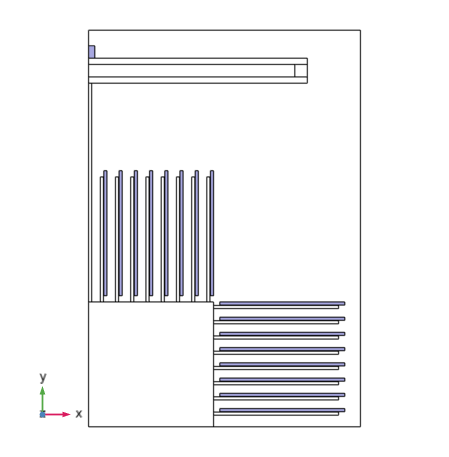
\includegraphics[width=1.0\linewidth]{fixed_boundaries.png}
            \caption{Fixed boundaries.}
            \label{fig:fixed-bound}
        \end{figure}
        
        All the other domains are set as \textbf{Free Linear Elastic Material}. To the \textit{polysilicon} domain, i.e. the whole structure, a \textbf{Body Load} was applied. The load was defined as a planar force per unit volume (\(N/m^3\)) with components:
        \begin{equation*}
            F_x=a_x g \rho_{poly}
        \end{equation*}
        \begin{equation*}
            F_y=a_y g \rho_{poly}
        \end{equation*}
        \begin{equation*}
            F_z=0
        \end{equation*}
        where \(g=9.81m/s^2\) is the gravity acceleration, whereas \(a_x\) and \(a_y\) are two model parameters. These are two pure numbers used to define the external acceleration as a multiple of \(g\).
        
        
        
        \bigskip
        \subsubsection{Electrostatics}
        In the \textit{Electrostatics} module, after applying the \textbf{Charge Conservation} to all the domains, air included, one horizontal and one vertical fingers were defined as \textbf{Terminals} of type \textit{Voltage}, with an applied voltage of \(1mV\). The fixed fingers boundaries that face those terminals were defined as \textbf{Ground} boundaries. This was necessary in order to evaluate the total equivalent capacitance between one pair of vertical/horizontal movable and fixed fingers. To include in the capacitance evaluation all the capacitances of a single movable-fixed fingers pair (two longitudinal and one transverse, see \ref{sssec:capacity}), the ground boundaries were selected as shown in figure \ref{fig:grounds}.
        
        \begin{figure}[!h]
            \centering
            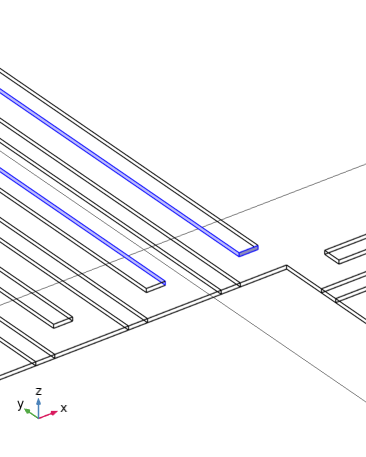
\includegraphics[width=1.0\linewidth]{grounds.png}
            \caption{Ground boundaries for one movable finger terminal.}
            \label{fig:grounds}
        \end{figure}
        
        The total X or Y differential capacitance can be simply obtained using equation ...
        
        The value of \(1mV\) applied to the terminals as a bias to sense the capacitance was chosen small enough so that electromechanical forces applied by the \textit{Multiphysics} module added only a negligible offset to the displacement of the mass.
        
        \bigskip
        \subsubsection{Multiphysics}
        The module used in this section is the \textbf{Electromechanical Forces}, which couples the \textit{Solid Mechanics} and \textit{Electrostatics} modules. Its settings were left as default.
        
        \bigskip
        \subsubsection{Mesh and Study}
        The used mesh was of type \textit{physics-controlled} with element size set to \textbf{coarse}, in order to follow what done by the authors of \cite{original}.
        
        Given that our interest is in the steady state of the system in different conditions, 4 \textbf{stationary} studies were defined:
        \begin{itemize}
            \item Parametric sweep of the parameter \(a_x\) (X axis acceleration) from \(1g\) to \(50g\) in 10 steps. \(a_y\) is set to 0 and the geometrical parameters are set to their default values, as specified in table \ref{tab:size}.
            \item Parametric sweep of the parameter \(a_y\) (Y axis acceleration) from \(1g\) to \(50g\) in 10 steps. \(a_x\) is set to 0 and the geometrical parameters are set to their default values, as specified in table \ref{tab:size}.
            \item Parametric sweep of the thickness of the straight beam \(t_{bx}\) from \(1\mu m\) to \(30\mu m\) in 20 steps. \(a_y\) is set to 0 and \(a_x\) is set to \(1g\), given that we need to find the displacement sensitivity along the X axis. The other geometrical parameters are set to their default values.
            \item Parametric sweep of the width of the straight beam \(w_{bx}\) from \(4\mu m\) to \(20\mu m\) in 20 steps. \(a_y\) is set to 0 and \(a_x\) is set to \(1g\), given that we need to find the displacement sensitivity along the X axis. The other geometrical parameters are set to their default values.
        \end{itemize}
        In all four studies, the \textit{direct stationary solver} and the \textit{suggested direct solver} were set to \textbf{MUMPS}.
        
    \subsection{Simulation Results}
    \subsubsection{\(a_x\) parametric sweep}
    The 3D plots for this simulation are presented in figures \ref{fig:disp_ax}, \ref{fig:disp_ax_det}, \ref{fig:stress_ax} and \ref{fig:stress_ax_det}.
     
    \begin{figure}[!h]
        \centering
        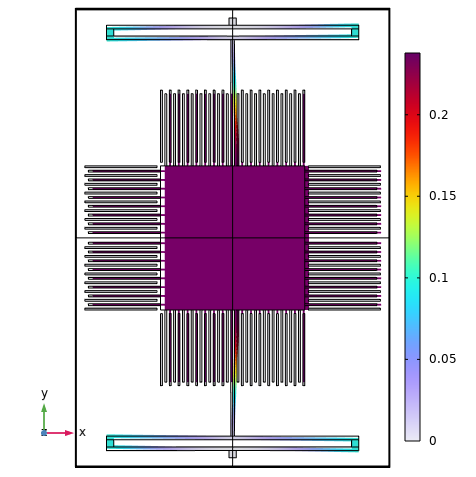
\includegraphics[width=1.0\linewidth]{displacement_ax}
        \caption{Displacement (\(\mu m\)) for acceleration \(a_x=50g\).}
        \label{fig:disp_ax}
    \end{figure}
    
    \begin{figure}[!h]
        \centering
        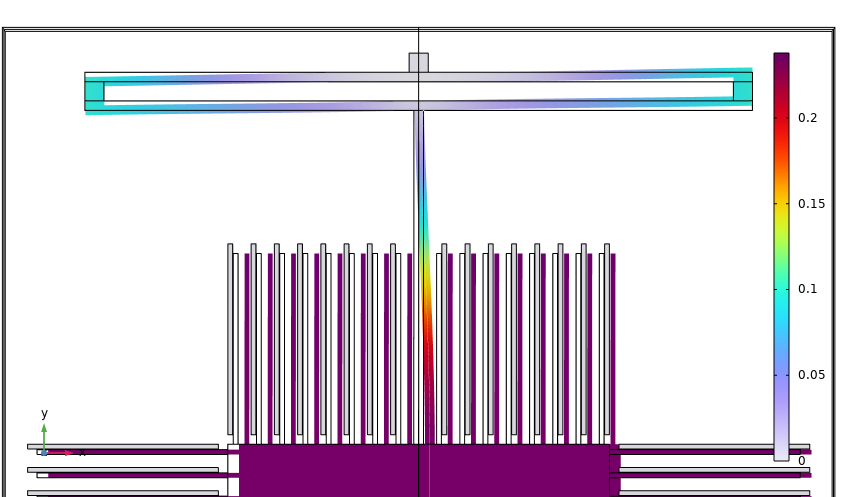
\includegraphics[width=1.0\linewidth]{displacement_ax_detail}
        \caption{Displacement (\(\mu m\)) for acceleration \(a_x=50g\), detail.}
        \label{fig:disp_ax_det}
    \end{figure}
    
    The maximum von Mises stress simulated for \(a_x=50g\) is \(4.2991\cdot10^6Pa\), which is almost identical to what is obtained in \cite{original} (\(4.5594\cdot10^6Pa\)). Therefore the conclusions are analogous: according to \cite{fracture}, the minimum fracture strength of polysilicon is \((2.9\pm 0.5)GPa\) (tensile stress), which is far higher then what we simulated at \(a_x=50g\), so there are no structural problems at this acceleration.
    
    \begin{figure}[!h]
        \centering
        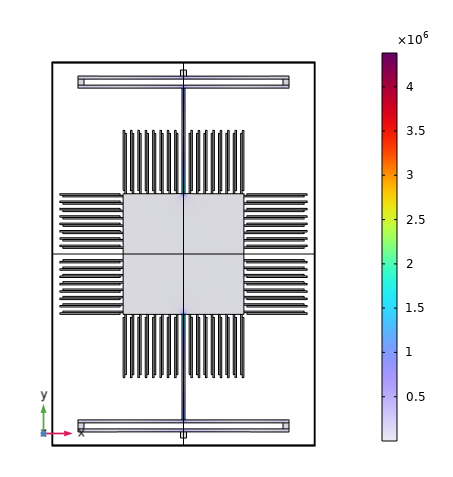
\includegraphics[width=1.0\linewidth]{stress_ax}
        \caption{Von Mises stress intensity (\(N/m^2\)) for acceleration \(a_x=50g\).}
        \label{fig:stress_ax}
    \end{figure}
    
    \begin{figure}[!h]
        \centering
        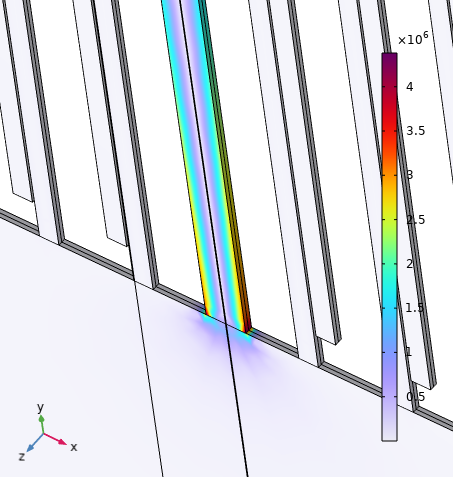
\includegraphics[width=1.0\linewidth]{stress_ax_detail}
        \caption{Von Mises stress intensity (\(N/m^2\)) for acceleration \(a_x=50g\), detail of the straight beam attachment to the central mass.}
        \label{fig:stress_ax_det}
    \end{figure}
    
    \begin{figure}
        \centering
        %% Creator: Matplotlib, PGF backend
%%
%% To include the figure in your LaTeX document, write
%%   \input{<filename>.pgf}
%%
%% Make sure the required packages are loaded in your preamble
%%   \usepackage{pgf}
%%
%% Also ensure that all the required font packages are loaded; for instance,
%% the lmodern package is sometimes necessary when using math font.
%%   \usepackage{lmodern}
%%
%% Figures using additional raster images can only be included by \input if
%% they are in the same directory as the main LaTeX file. For loading figures
%% from other directories you can use the `import` package
%%   \usepackage{import}
%%
%% and then include the figures with
%%   \import{<path to file>}{<filename>.pgf}
%%
%% Matplotlib used the following preamble
%%   \def\mathdefault#1{#1}
%%   \everymath=\expandafter{\the\everymath\displaystyle}
%%   \IfFileExists{scrextend.sty}{
%%     \usepackage[fontsize=10.000000pt]{scrextend}
%%   }{
%%     \renewcommand{\normalsize}{\fontsize{10.000000}{12.000000}\selectfont}
%%     \normalsize
%%   }
%%   
%%   \ifdefined\pdftexversion\else  % non-pdftex case.
%%     \usepackage{fontspec}
%%     \setmainfont{DejaVuSerif.ttf}[Path=\detokenize{C:/Users/leona/Desktop/dual_axis_accelerometer/python/Lib/site-packages/matplotlib/mpl-data/fonts/ttf/}]
%%     \setsansfont{DejaVuSans.ttf}[Path=\detokenize{C:/Users/leona/Desktop/dual_axis_accelerometer/python/Lib/site-packages/matplotlib/mpl-data/fonts/ttf/}]
%%     \setmonofont{DejaVuSansMono.ttf}[Path=\detokenize{C:/Users/leona/Desktop/dual_axis_accelerometer/python/Lib/site-packages/matplotlib/mpl-data/fonts/ttf/}]
%%   \fi
%%   \makeatletter\@ifpackageloaded{underscore}{}{\usepackage[strings]{underscore}}\makeatother
%%
\begingroup%
\makeatletter%
\begin{pgfpicture}%
\pgfpathrectangle{\pgfpointorigin}{\pgfqpoint{6.400000in}{4.800000in}}%
\pgfusepath{use as bounding box, clip}%
\begin{pgfscope}%
\pgfsetbuttcap%
\pgfsetmiterjoin%
\definecolor{currentfill}{rgb}{1.000000,1.000000,1.000000}%
\pgfsetfillcolor{currentfill}%
\pgfsetlinewidth{0.000000pt}%
\definecolor{currentstroke}{rgb}{1.000000,1.000000,1.000000}%
\pgfsetstrokecolor{currentstroke}%
\pgfsetdash{}{0pt}%
\pgfpathmoveto{\pgfqpoint{0.000000in}{0.000000in}}%
\pgfpathlineto{\pgfqpoint{6.400000in}{0.000000in}}%
\pgfpathlineto{\pgfqpoint{6.400000in}{4.800000in}}%
\pgfpathlineto{\pgfqpoint{0.000000in}{4.800000in}}%
\pgfpathlineto{\pgfqpoint{0.000000in}{0.000000in}}%
\pgfpathclose%
\pgfusepath{fill}%
\end{pgfscope}%
\begin{pgfscope}%
\pgfsetbuttcap%
\pgfsetmiterjoin%
\definecolor{currentfill}{rgb}{1.000000,1.000000,1.000000}%
\pgfsetfillcolor{currentfill}%
\pgfsetlinewidth{0.000000pt}%
\definecolor{currentstroke}{rgb}{0.000000,0.000000,0.000000}%
\pgfsetstrokecolor{currentstroke}%
\pgfsetstrokeopacity{0.000000}%
\pgfsetdash{}{0pt}%
\pgfpathmoveto{\pgfqpoint{0.800000in}{0.528000in}}%
\pgfpathlineto{\pgfqpoint{5.760000in}{0.528000in}}%
\pgfpathlineto{\pgfqpoint{5.760000in}{4.224000in}}%
\pgfpathlineto{\pgfqpoint{0.800000in}{4.224000in}}%
\pgfpathlineto{\pgfqpoint{0.800000in}{0.528000in}}%
\pgfpathclose%
\pgfusepath{fill}%
\end{pgfscope}%
\begin{pgfscope}%
\pgfpathrectangle{\pgfqpoint{0.800000in}{0.528000in}}{\pgfqpoint{4.960000in}{3.696000in}}%
\pgfusepath{clip}%
\pgfsetrectcap%
\pgfsetroundjoin%
\pgfsetlinewidth{0.803000pt}%
\definecolor{currentstroke}{rgb}{0.690196,0.690196,0.690196}%
\pgfsetstrokecolor{currentstroke}%
\pgfsetdash{}{0pt}%
\pgfpathmoveto{\pgfqpoint{0.933432in}{0.528000in}}%
\pgfpathlineto{\pgfqpoint{0.933432in}{4.224000in}}%
\pgfusepath{stroke}%
\end{pgfscope}%
\begin{pgfscope}%
\pgfsetbuttcap%
\pgfsetroundjoin%
\definecolor{currentfill}{rgb}{0.000000,0.000000,0.000000}%
\pgfsetfillcolor{currentfill}%
\pgfsetlinewidth{0.803000pt}%
\definecolor{currentstroke}{rgb}{0.000000,0.000000,0.000000}%
\pgfsetstrokecolor{currentstroke}%
\pgfsetdash{}{0pt}%
\pgfsys@defobject{currentmarker}{\pgfqpoint{0.000000in}{-0.048611in}}{\pgfqpoint{0.000000in}{0.000000in}}{%
\pgfpathmoveto{\pgfqpoint{0.000000in}{0.000000in}}%
\pgfpathlineto{\pgfqpoint{0.000000in}{-0.048611in}}%
\pgfusepath{stroke,fill}%
}%
\begin{pgfscope}%
\pgfsys@transformshift{0.933432in}{0.528000in}%
\pgfsys@useobject{currentmarker}{}%
\end{pgfscope}%
\end{pgfscope}%
\begin{pgfscope}%
\definecolor{textcolor}{rgb}{0.000000,0.000000,0.000000}%
\pgfsetstrokecolor{textcolor}%
\pgfsetfillcolor{textcolor}%
\pgftext[x=0.933432in,y=0.430778in,,top]{\color{textcolor}{\sffamily\fontsize{10.000000}{12.000000}\selectfont\catcode`\^=\active\def^{\ifmmode\sp\else\^{}\fi}\catcode`\%=\active\def%{\%}0}}%
\end{pgfscope}%
\begin{pgfscope}%
\pgfpathrectangle{\pgfqpoint{0.800000in}{0.528000in}}{\pgfqpoint{4.960000in}{3.696000in}}%
\pgfusepath{clip}%
\pgfsetrectcap%
\pgfsetroundjoin%
\pgfsetlinewidth{0.803000pt}%
\definecolor{currentstroke}{rgb}{0.690196,0.690196,0.690196}%
\pgfsetstrokecolor{currentstroke}%
\pgfsetdash{}{0pt}%
\pgfpathmoveto{\pgfqpoint{1.853655in}{0.528000in}}%
\pgfpathlineto{\pgfqpoint{1.853655in}{4.224000in}}%
\pgfusepath{stroke}%
\end{pgfscope}%
\begin{pgfscope}%
\pgfsetbuttcap%
\pgfsetroundjoin%
\definecolor{currentfill}{rgb}{0.000000,0.000000,0.000000}%
\pgfsetfillcolor{currentfill}%
\pgfsetlinewidth{0.803000pt}%
\definecolor{currentstroke}{rgb}{0.000000,0.000000,0.000000}%
\pgfsetstrokecolor{currentstroke}%
\pgfsetdash{}{0pt}%
\pgfsys@defobject{currentmarker}{\pgfqpoint{0.000000in}{-0.048611in}}{\pgfqpoint{0.000000in}{0.000000in}}{%
\pgfpathmoveto{\pgfqpoint{0.000000in}{0.000000in}}%
\pgfpathlineto{\pgfqpoint{0.000000in}{-0.048611in}}%
\pgfusepath{stroke,fill}%
}%
\begin{pgfscope}%
\pgfsys@transformshift{1.853655in}{0.528000in}%
\pgfsys@useobject{currentmarker}{}%
\end{pgfscope}%
\end{pgfscope}%
\begin{pgfscope}%
\definecolor{textcolor}{rgb}{0.000000,0.000000,0.000000}%
\pgfsetstrokecolor{textcolor}%
\pgfsetfillcolor{textcolor}%
\pgftext[x=1.853655in,y=0.430778in,,top]{\color{textcolor}{\sffamily\fontsize{10.000000}{12.000000}\selectfont\catcode`\^=\active\def^{\ifmmode\sp\else\^{}\fi}\catcode`\%=\active\def%{\%}10}}%
\end{pgfscope}%
\begin{pgfscope}%
\pgfpathrectangle{\pgfqpoint{0.800000in}{0.528000in}}{\pgfqpoint{4.960000in}{3.696000in}}%
\pgfusepath{clip}%
\pgfsetrectcap%
\pgfsetroundjoin%
\pgfsetlinewidth{0.803000pt}%
\definecolor{currentstroke}{rgb}{0.690196,0.690196,0.690196}%
\pgfsetstrokecolor{currentstroke}%
\pgfsetdash{}{0pt}%
\pgfpathmoveto{\pgfqpoint{2.773878in}{0.528000in}}%
\pgfpathlineto{\pgfqpoint{2.773878in}{4.224000in}}%
\pgfusepath{stroke}%
\end{pgfscope}%
\begin{pgfscope}%
\pgfsetbuttcap%
\pgfsetroundjoin%
\definecolor{currentfill}{rgb}{0.000000,0.000000,0.000000}%
\pgfsetfillcolor{currentfill}%
\pgfsetlinewidth{0.803000pt}%
\definecolor{currentstroke}{rgb}{0.000000,0.000000,0.000000}%
\pgfsetstrokecolor{currentstroke}%
\pgfsetdash{}{0pt}%
\pgfsys@defobject{currentmarker}{\pgfqpoint{0.000000in}{-0.048611in}}{\pgfqpoint{0.000000in}{0.000000in}}{%
\pgfpathmoveto{\pgfqpoint{0.000000in}{0.000000in}}%
\pgfpathlineto{\pgfqpoint{0.000000in}{-0.048611in}}%
\pgfusepath{stroke,fill}%
}%
\begin{pgfscope}%
\pgfsys@transformshift{2.773878in}{0.528000in}%
\pgfsys@useobject{currentmarker}{}%
\end{pgfscope}%
\end{pgfscope}%
\begin{pgfscope}%
\definecolor{textcolor}{rgb}{0.000000,0.000000,0.000000}%
\pgfsetstrokecolor{textcolor}%
\pgfsetfillcolor{textcolor}%
\pgftext[x=2.773878in,y=0.430778in,,top]{\color{textcolor}{\sffamily\fontsize{10.000000}{12.000000}\selectfont\catcode`\^=\active\def^{\ifmmode\sp\else\^{}\fi}\catcode`\%=\active\def%{\%}20}}%
\end{pgfscope}%
\begin{pgfscope}%
\pgfpathrectangle{\pgfqpoint{0.800000in}{0.528000in}}{\pgfqpoint{4.960000in}{3.696000in}}%
\pgfusepath{clip}%
\pgfsetrectcap%
\pgfsetroundjoin%
\pgfsetlinewidth{0.803000pt}%
\definecolor{currentstroke}{rgb}{0.690196,0.690196,0.690196}%
\pgfsetstrokecolor{currentstroke}%
\pgfsetdash{}{0pt}%
\pgfpathmoveto{\pgfqpoint{3.694100in}{0.528000in}}%
\pgfpathlineto{\pgfqpoint{3.694100in}{4.224000in}}%
\pgfusepath{stroke}%
\end{pgfscope}%
\begin{pgfscope}%
\pgfsetbuttcap%
\pgfsetroundjoin%
\definecolor{currentfill}{rgb}{0.000000,0.000000,0.000000}%
\pgfsetfillcolor{currentfill}%
\pgfsetlinewidth{0.803000pt}%
\definecolor{currentstroke}{rgb}{0.000000,0.000000,0.000000}%
\pgfsetstrokecolor{currentstroke}%
\pgfsetdash{}{0pt}%
\pgfsys@defobject{currentmarker}{\pgfqpoint{0.000000in}{-0.048611in}}{\pgfqpoint{0.000000in}{0.000000in}}{%
\pgfpathmoveto{\pgfqpoint{0.000000in}{0.000000in}}%
\pgfpathlineto{\pgfqpoint{0.000000in}{-0.048611in}}%
\pgfusepath{stroke,fill}%
}%
\begin{pgfscope}%
\pgfsys@transformshift{3.694100in}{0.528000in}%
\pgfsys@useobject{currentmarker}{}%
\end{pgfscope}%
\end{pgfscope}%
\begin{pgfscope}%
\definecolor{textcolor}{rgb}{0.000000,0.000000,0.000000}%
\pgfsetstrokecolor{textcolor}%
\pgfsetfillcolor{textcolor}%
\pgftext[x=3.694100in,y=0.430778in,,top]{\color{textcolor}{\sffamily\fontsize{10.000000}{12.000000}\selectfont\catcode`\^=\active\def^{\ifmmode\sp\else\^{}\fi}\catcode`\%=\active\def%{\%}30}}%
\end{pgfscope}%
\begin{pgfscope}%
\pgfpathrectangle{\pgfqpoint{0.800000in}{0.528000in}}{\pgfqpoint{4.960000in}{3.696000in}}%
\pgfusepath{clip}%
\pgfsetrectcap%
\pgfsetroundjoin%
\pgfsetlinewidth{0.803000pt}%
\definecolor{currentstroke}{rgb}{0.690196,0.690196,0.690196}%
\pgfsetstrokecolor{currentstroke}%
\pgfsetdash{}{0pt}%
\pgfpathmoveto{\pgfqpoint{4.614323in}{0.528000in}}%
\pgfpathlineto{\pgfqpoint{4.614323in}{4.224000in}}%
\pgfusepath{stroke}%
\end{pgfscope}%
\begin{pgfscope}%
\pgfsetbuttcap%
\pgfsetroundjoin%
\definecolor{currentfill}{rgb}{0.000000,0.000000,0.000000}%
\pgfsetfillcolor{currentfill}%
\pgfsetlinewidth{0.803000pt}%
\definecolor{currentstroke}{rgb}{0.000000,0.000000,0.000000}%
\pgfsetstrokecolor{currentstroke}%
\pgfsetdash{}{0pt}%
\pgfsys@defobject{currentmarker}{\pgfqpoint{0.000000in}{-0.048611in}}{\pgfqpoint{0.000000in}{0.000000in}}{%
\pgfpathmoveto{\pgfqpoint{0.000000in}{0.000000in}}%
\pgfpathlineto{\pgfqpoint{0.000000in}{-0.048611in}}%
\pgfusepath{stroke,fill}%
}%
\begin{pgfscope}%
\pgfsys@transformshift{4.614323in}{0.528000in}%
\pgfsys@useobject{currentmarker}{}%
\end{pgfscope}%
\end{pgfscope}%
\begin{pgfscope}%
\definecolor{textcolor}{rgb}{0.000000,0.000000,0.000000}%
\pgfsetstrokecolor{textcolor}%
\pgfsetfillcolor{textcolor}%
\pgftext[x=4.614323in,y=0.430778in,,top]{\color{textcolor}{\sffamily\fontsize{10.000000}{12.000000}\selectfont\catcode`\^=\active\def^{\ifmmode\sp\else\^{}\fi}\catcode`\%=\active\def%{\%}40}}%
\end{pgfscope}%
\begin{pgfscope}%
\pgfpathrectangle{\pgfqpoint{0.800000in}{0.528000in}}{\pgfqpoint{4.960000in}{3.696000in}}%
\pgfusepath{clip}%
\pgfsetrectcap%
\pgfsetroundjoin%
\pgfsetlinewidth{0.803000pt}%
\definecolor{currentstroke}{rgb}{0.690196,0.690196,0.690196}%
\pgfsetstrokecolor{currentstroke}%
\pgfsetdash{}{0pt}%
\pgfpathmoveto{\pgfqpoint{5.534545in}{0.528000in}}%
\pgfpathlineto{\pgfqpoint{5.534545in}{4.224000in}}%
\pgfusepath{stroke}%
\end{pgfscope}%
\begin{pgfscope}%
\pgfsetbuttcap%
\pgfsetroundjoin%
\definecolor{currentfill}{rgb}{0.000000,0.000000,0.000000}%
\pgfsetfillcolor{currentfill}%
\pgfsetlinewidth{0.803000pt}%
\definecolor{currentstroke}{rgb}{0.000000,0.000000,0.000000}%
\pgfsetstrokecolor{currentstroke}%
\pgfsetdash{}{0pt}%
\pgfsys@defobject{currentmarker}{\pgfqpoint{0.000000in}{-0.048611in}}{\pgfqpoint{0.000000in}{0.000000in}}{%
\pgfpathmoveto{\pgfqpoint{0.000000in}{0.000000in}}%
\pgfpathlineto{\pgfqpoint{0.000000in}{-0.048611in}}%
\pgfusepath{stroke,fill}%
}%
\begin{pgfscope}%
\pgfsys@transformshift{5.534545in}{0.528000in}%
\pgfsys@useobject{currentmarker}{}%
\end{pgfscope}%
\end{pgfscope}%
\begin{pgfscope}%
\definecolor{textcolor}{rgb}{0.000000,0.000000,0.000000}%
\pgfsetstrokecolor{textcolor}%
\pgfsetfillcolor{textcolor}%
\pgftext[x=5.534545in,y=0.430778in,,top]{\color{textcolor}{\sffamily\fontsize{10.000000}{12.000000}\selectfont\catcode`\^=\active\def^{\ifmmode\sp\else\^{}\fi}\catcode`\%=\active\def%{\%}50}}%
\end{pgfscope}%
\begin{pgfscope}%
\definecolor{textcolor}{rgb}{0.000000,0.000000,0.000000}%
\pgfsetstrokecolor{textcolor}%
\pgfsetfillcolor{textcolor}%
\pgftext[x=3.280000in,y=0.240809in,,top]{\color{textcolor}{\sffamily\fontsize{10.000000}{12.000000}\selectfont\catcode`\^=\active\def^{\ifmmode\sp\else\^{}\fi}\catcode`\%=\active\def%{\%}X axis acceleration $a_x$ (g)}}%
\end{pgfscope}%
\begin{pgfscope}%
\pgfpathrectangle{\pgfqpoint{0.800000in}{0.528000in}}{\pgfqpoint{4.960000in}{3.696000in}}%
\pgfusepath{clip}%
\pgfsetrectcap%
\pgfsetroundjoin%
\pgfsetlinewidth{0.803000pt}%
\definecolor{currentstroke}{rgb}{0.690196,0.690196,0.690196}%
\pgfsetstrokecolor{currentstroke}%
\pgfsetdash{}{0pt}%
\pgfpathmoveto{\pgfqpoint{0.800000in}{0.627355in}}%
\pgfpathlineto{\pgfqpoint{5.760000in}{0.627355in}}%
\pgfusepath{stroke}%
\end{pgfscope}%
\begin{pgfscope}%
\pgfsetbuttcap%
\pgfsetroundjoin%
\definecolor{currentfill}{rgb}{0.000000,0.000000,0.000000}%
\pgfsetfillcolor{currentfill}%
\pgfsetlinewidth{0.803000pt}%
\definecolor{currentstroke}{rgb}{0.000000,0.000000,0.000000}%
\pgfsetstrokecolor{currentstroke}%
\pgfsetdash{}{0pt}%
\pgfsys@defobject{currentmarker}{\pgfqpoint{-0.048611in}{0.000000in}}{\pgfqpoint{-0.000000in}{0.000000in}}{%
\pgfpathmoveto{\pgfqpoint{-0.000000in}{0.000000in}}%
\pgfpathlineto{\pgfqpoint{-0.048611in}{0.000000in}}%
\pgfusepath{stroke,fill}%
}%
\begin{pgfscope}%
\pgfsys@transformshift{0.800000in}{0.627355in}%
\pgfsys@useobject{currentmarker}{}%
\end{pgfscope}%
\end{pgfscope}%
\begin{pgfscope}%
\definecolor{textcolor}{rgb}{0.000000,0.000000,0.000000}%
\pgfsetstrokecolor{textcolor}%
\pgfsetfillcolor{textcolor}%
\pgftext[x=0.393533in, y=0.574593in, left, base]{\color{textcolor}{\sffamily\fontsize{10.000000}{12.000000}\selectfont\catcode`\^=\active\def^{\ifmmode\sp\else\^{}\fi}\catcode`\%=\active\def%{\%}0.00}}%
\end{pgfscope}%
\begin{pgfscope}%
\pgfpathrectangle{\pgfqpoint{0.800000in}{0.528000in}}{\pgfqpoint{4.960000in}{3.696000in}}%
\pgfusepath{clip}%
\pgfsetrectcap%
\pgfsetroundjoin%
\pgfsetlinewidth{0.803000pt}%
\definecolor{currentstroke}{rgb}{0.690196,0.690196,0.690196}%
\pgfsetstrokecolor{currentstroke}%
\pgfsetdash{}{0pt}%
\pgfpathmoveto{\pgfqpoint{0.800000in}{1.348180in}}%
\pgfpathlineto{\pgfqpoint{5.760000in}{1.348180in}}%
\pgfusepath{stroke}%
\end{pgfscope}%
\begin{pgfscope}%
\pgfsetbuttcap%
\pgfsetroundjoin%
\definecolor{currentfill}{rgb}{0.000000,0.000000,0.000000}%
\pgfsetfillcolor{currentfill}%
\pgfsetlinewidth{0.803000pt}%
\definecolor{currentstroke}{rgb}{0.000000,0.000000,0.000000}%
\pgfsetstrokecolor{currentstroke}%
\pgfsetdash{}{0pt}%
\pgfsys@defobject{currentmarker}{\pgfqpoint{-0.048611in}{0.000000in}}{\pgfqpoint{-0.000000in}{0.000000in}}{%
\pgfpathmoveto{\pgfqpoint{-0.000000in}{0.000000in}}%
\pgfpathlineto{\pgfqpoint{-0.048611in}{0.000000in}}%
\pgfusepath{stroke,fill}%
}%
\begin{pgfscope}%
\pgfsys@transformshift{0.800000in}{1.348180in}%
\pgfsys@useobject{currentmarker}{}%
\end{pgfscope}%
\end{pgfscope}%
\begin{pgfscope}%
\definecolor{textcolor}{rgb}{0.000000,0.000000,0.000000}%
\pgfsetstrokecolor{textcolor}%
\pgfsetfillcolor{textcolor}%
\pgftext[x=0.393533in, y=1.295419in, left, base]{\color{textcolor}{\sffamily\fontsize{10.000000}{12.000000}\selectfont\catcode`\^=\active\def^{\ifmmode\sp\else\^{}\fi}\catcode`\%=\active\def%{\%}0.05}}%
\end{pgfscope}%
\begin{pgfscope}%
\pgfpathrectangle{\pgfqpoint{0.800000in}{0.528000in}}{\pgfqpoint{4.960000in}{3.696000in}}%
\pgfusepath{clip}%
\pgfsetrectcap%
\pgfsetroundjoin%
\pgfsetlinewidth{0.803000pt}%
\definecolor{currentstroke}{rgb}{0.690196,0.690196,0.690196}%
\pgfsetstrokecolor{currentstroke}%
\pgfsetdash{}{0pt}%
\pgfpathmoveto{\pgfqpoint{0.800000in}{2.069005in}}%
\pgfpathlineto{\pgfqpoint{5.760000in}{2.069005in}}%
\pgfusepath{stroke}%
\end{pgfscope}%
\begin{pgfscope}%
\pgfsetbuttcap%
\pgfsetroundjoin%
\definecolor{currentfill}{rgb}{0.000000,0.000000,0.000000}%
\pgfsetfillcolor{currentfill}%
\pgfsetlinewidth{0.803000pt}%
\definecolor{currentstroke}{rgb}{0.000000,0.000000,0.000000}%
\pgfsetstrokecolor{currentstroke}%
\pgfsetdash{}{0pt}%
\pgfsys@defobject{currentmarker}{\pgfqpoint{-0.048611in}{0.000000in}}{\pgfqpoint{-0.000000in}{0.000000in}}{%
\pgfpathmoveto{\pgfqpoint{-0.000000in}{0.000000in}}%
\pgfpathlineto{\pgfqpoint{-0.048611in}{0.000000in}}%
\pgfusepath{stroke,fill}%
}%
\begin{pgfscope}%
\pgfsys@transformshift{0.800000in}{2.069005in}%
\pgfsys@useobject{currentmarker}{}%
\end{pgfscope}%
\end{pgfscope}%
\begin{pgfscope}%
\definecolor{textcolor}{rgb}{0.000000,0.000000,0.000000}%
\pgfsetstrokecolor{textcolor}%
\pgfsetfillcolor{textcolor}%
\pgftext[x=0.393533in, y=2.016244in, left, base]{\color{textcolor}{\sffamily\fontsize{10.000000}{12.000000}\selectfont\catcode`\^=\active\def^{\ifmmode\sp\else\^{}\fi}\catcode`\%=\active\def%{\%}0.10}}%
\end{pgfscope}%
\begin{pgfscope}%
\pgfpathrectangle{\pgfqpoint{0.800000in}{0.528000in}}{\pgfqpoint{4.960000in}{3.696000in}}%
\pgfusepath{clip}%
\pgfsetrectcap%
\pgfsetroundjoin%
\pgfsetlinewidth{0.803000pt}%
\definecolor{currentstroke}{rgb}{0.690196,0.690196,0.690196}%
\pgfsetstrokecolor{currentstroke}%
\pgfsetdash{}{0pt}%
\pgfpathmoveto{\pgfqpoint{0.800000in}{2.789830in}}%
\pgfpathlineto{\pgfqpoint{5.760000in}{2.789830in}}%
\pgfusepath{stroke}%
\end{pgfscope}%
\begin{pgfscope}%
\pgfsetbuttcap%
\pgfsetroundjoin%
\definecolor{currentfill}{rgb}{0.000000,0.000000,0.000000}%
\pgfsetfillcolor{currentfill}%
\pgfsetlinewidth{0.803000pt}%
\definecolor{currentstroke}{rgb}{0.000000,0.000000,0.000000}%
\pgfsetstrokecolor{currentstroke}%
\pgfsetdash{}{0pt}%
\pgfsys@defobject{currentmarker}{\pgfqpoint{-0.048611in}{0.000000in}}{\pgfqpoint{-0.000000in}{0.000000in}}{%
\pgfpathmoveto{\pgfqpoint{-0.000000in}{0.000000in}}%
\pgfpathlineto{\pgfqpoint{-0.048611in}{0.000000in}}%
\pgfusepath{stroke,fill}%
}%
\begin{pgfscope}%
\pgfsys@transformshift{0.800000in}{2.789830in}%
\pgfsys@useobject{currentmarker}{}%
\end{pgfscope}%
\end{pgfscope}%
\begin{pgfscope}%
\definecolor{textcolor}{rgb}{0.000000,0.000000,0.000000}%
\pgfsetstrokecolor{textcolor}%
\pgfsetfillcolor{textcolor}%
\pgftext[x=0.393533in, y=2.737069in, left, base]{\color{textcolor}{\sffamily\fontsize{10.000000}{12.000000}\selectfont\catcode`\^=\active\def^{\ifmmode\sp\else\^{}\fi}\catcode`\%=\active\def%{\%}0.15}}%
\end{pgfscope}%
\begin{pgfscope}%
\pgfpathrectangle{\pgfqpoint{0.800000in}{0.528000in}}{\pgfqpoint{4.960000in}{3.696000in}}%
\pgfusepath{clip}%
\pgfsetrectcap%
\pgfsetroundjoin%
\pgfsetlinewidth{0.803000pt}%
\definecolor{currentstroke}{rgb}{0.690196,0.690196,0.690196}%
\pgfsetstrokecolor{currentstroke}%
\pgfsetdash{}{0pt}%
\pgfpathmoveto{\pgfqpoint{0.800000in}{3.510656in}}%
\pgfpathlineto{\pgfqpoint{5.760000in}{3.510656in}}%
\pgfusepath{stroke}%
\end{pgfscope}%
\begin{pgfscope}%
\pgfsetbuttcap%
\pgfsetroundjoin%
\definecolor{currentfill}{rgb}{0.000000,0.000000,0.000000}%
\pgfsetfillcolor{currentfill}%
\pgfsetlinewidth{0.803000pt}%
\definecolor{currentstroke}{rgb}{0.000000,0.000000,0.000000}%
\pgfsetstrokecolor{currentstroke}%
\pgfsetdash{}{0pt}%
\pgfsys@defobject{currentmarker}{\pgfqpoint{-0.048611in}{0.000000in}}{\pgfqpoint{-0.000000in}{0.000000in}}{%
\pgfpathmoveto{\pgfqpoint{-0.000000in}{0.000000in}}%
\pgfpathlineto{\pgfqpoint{-0.048611in}{0.000000in}}%
\pgfusepath{stroke,fill}%
}%
\begin{pgfscope}%
\pgfsys@transformshift{0.800000in}{3.510656in}%
\pgfsys@useobject{currentmarker}{}%
\end{pgfscope}%
\end{pgfscope}%
\begin{pgfscope}%
\definecolor{textcolor}{rgb}{0.000000,0.000000,0.000000}%
\pgfsetstrokecolor{textcolor}%
\pgfsetfillcolor{textcolor}%
\pgftext[x=0.393533in, y=3.457894in, left, base]{\color{textcolor}{\sffamily\fontsize{10.000000}{12.000000}\selectfont\catcode`\^=\active\def^{\ifmmode\sp\else\^{}\fi}\catcode`\%=\active\def%{\%}0.20}}%
\end{pgfscope}%
\begin{pgfscope}%
\definecolor{textcolor}{rgb}{0.000000,0.000000,0.000000}%
\pgfsetstrokecolor{textcolor}%
\pgfsetfillcolor{textcolor}%
\pgftext[x=0.337977in,y=2.376000in,,bottom,rotate=90.000000]{\color{textcolor}{\sffamily\fontsize{10.000000}{12.000000}\selectfont\catcode`\^=\active\def^{\ifmmode\sp\else\^{}\fi}\catcode`\%=\active\def%{\%}Max displacement along X axis}}%
\end{pgfscope}%
\begin{pgfscope}%
\pgfpathrectangle{\pgfqpoint{0.800000in}{0.528000in}}{\pgfqpoint{4.960000in}{3.696000in}}%
\pgfusepath{clip}%
\pgfsetrectcap%
\pgfsetroundjoin%
\pgfsetlinewidth{1.505625pt}%
\definecolor{currentstroke}{rgb}{0.121569,0.466667,0.705882}%
\pgfsetstrokecolor{currentstroke}%
\pgfsetdash{}{0pt}%
\pgfpathmoveto{\pgfqpoint{1.025455in}{0.696000in}}%
\pgfpathlineto{\pgfqpoint{1.526465in}{1.069689in}}%
\pgfpathlineto{\pgfqpoint{2.027475in}{1.443298in}}%
\pgfpathlineto{\pgfqpoint{2.528485in}{1.816824in}}%
\pgfpathlineto{\pgfqpoint{3.029495in}{2.190262in}}%
\pgfpathlineto{\pgfqpoint{3.530505in}{2.563608in}}%
\pgfpathlineto{\pgfqpoint{4.031515in}{2.936859in}}%
\pgfpathlineto{\pgfqpoint{4.532525in}{3.310011in}}%
\pgfpathlineto{\pgfqpoint{5.033535in}{3.683059in}}%
\pgfpathlineto{\pgfqpoint{5.534545in}{4.056000in}}%
\pgfusepath{stroke}%
\end{pgfscope}%
\begin{pgfscope}%
\pgfpathrectangle{\pgfqpoint{0.800000in}{0.528000in}}{\pgfqpoint{4.960000in}{3.696000in}}%
\pgfusepath{clip}%
\pgfsetbuttcap%
\pgfsetroundjoin%
\definecolor{currentfill}{rgb}{0.121569,0.466667,0.705882}%
\pgfsetfillcolor{currentfill}%
\pgfsetlinewidth{1.003750pt}%
\definecolor{currentstroke}{rgb}{0.121569,0.466667,0.705882}%
\pgfsetstrokecolor{currentstroke}%
\pgfsetdash{}{0pt}%
\pgfsys@defobject{currentmarker}{\pgfqpoint{-0.041667in}{-0.041667in}}{\pgfqpoint{0.041667in}{0.041667in}}{%
\pgfpathmoveto{\pgfqpoint{0.000000in}{-0.041667in}}%
\pgfpathcurveto{\pgfqpoint{0.011050in}{-0.041667in}}{\pgfqpoint{0.021649in}{-0.037276in}}{\pgfqpoint{0.029463in}{-0.029463in}}%
\pgfpathcurveto{\pgfqpoint{0.037276in}{-0.021649in}}{\pgfqpoint{0.041667in}{-0.011050in}}{\pgfqpoint{0.041667in}{0.000000in}}%
\pgfpathcurveto{\pgfqpoint{0.041667in}{0.011050in}}{\pgfqpoint{0.037276in}{0.021649in}}{\pgfqpoint{0.029463in}{0.029463in}}%
\pgfpathcurveto{\pgfqpoint{0.021649in}{0.037276in}}{\pgfqpoint{0.011050in}{0.041667in}}{\pgfqpoint{0.000000in}{0.041667in}}%
\pgfpathcurveto{\pgfqpoint{-0.011050in}{0.041667in}}{\pgfqpoint{-0.021649in}{0.037276in}}{\pgfqpoint{-0.029463in}{0.029463in}}%
\pgfpathcurveto{\pgfqpoint{-0.037276in}{0.021649in}}{\pgfqpoint{-0.041667in}{0.011050in}}{\pgfqpoint{-0.041667in}{0.000000in}}%
\pgfpathcurveto{\pgfqpoint{-0.041667in}{-0.011050in}}{\pgfqpoint{-0.037276in}{-0.021649in}}{\pgfqpoint{-0.029463in}{-0.029463in}}%
\pgfpathcurveto{\pgfqpoint{-0.021649in}{-0.037276in}}{\pgfqpoint{-0.011050in}{-0.041667in}}{\pgfqpoint{0.000000in}{-0.041667in}}%
\pgfpathlineto{\pgfqpoint{0.000000in}{-0.041667in}}%
\pgfpathclose%
\pgfusepath{stroke,fill}%
}%
\begin{pgfscope}%
\pgfsys@transformshift{1.025455in}{0.696000in}%
\pgfsys@useobject{currentmarker}{}%
\end{pgfscope}%
\begin{pgfscope}%
\pgfsys@transformshift{1.526465in}{1.069689in}%
\pgfsys@useobject{currentmarker}{}%
\end{pgfscope}%
\begin{pgfscope}%
\pgfsys@transformshift{2.027475in}{1.443298in}%
\pgfsys@useobject{currentmarker}{}%
\end{pgfscope}%
\begin{pgfscope}%
\pgfsys@transformshift{2.528485in}{1.816824in}%
\pgfsys@useobject{currentmarker}{}%
\end{pgfscope}%
\begin{pgfscope}%
\pgfsys@transformshift{3.029495in}{2.190262in}%
\pgfsys@useobject{currentmarker}{}%
\end{pgfscope}%
\begin{pgfscope}%
\pgfsys@transformshift{3.530505in}{2.563608in}%
\pgfsys@useobject{currentmarker}{}%
\end{pgfscope}%
\begin{pgfscope}%
\pgfsys@transformshift{4.031515in}{2.936859in}%
\pgfsys@useobject{currentmarker}{}%
\end{pgfscope}%
\begin{pgfscope}%
\pgfsys@transformshift{4.532525in}{3.310011in}%
\pgfsys@useobject{currentmarker}{}%
\end{pgfscope}%
\begin{pgfscope}%
\pgfsys@transformshift{5.033535in}{3.683059in}%
\pgfsys@useobject{currentmarker}{}%
\end{pgfscope}%
\begin{pgfscope}%
\pgfsys@transformshift{5.534545in}{4.056000in}%
\pgfsys@useobject{currentmarker}{}%
\end{pgfscope}%
\end{pgfscope}%
\begin{pgfscope}%
\pgfsetrectcap%
\pgfsetmiterjoin%
\pgfsetlinewidth{0.803000pt}%
\definecolor{currentstroke}{rgb}{0.000000,0.000000,0.000000}%
\pgfsetstrokecolor{currentstroke}%
\pgfsetdash{}{0pt}%
\pgfpathmoveto{\pgfqpoint{0.800000in}{0.528000in}}%
\pgfpathlineto{\pgfqpoint{0.800000in}{4.224000in}}%
\pgfusepath{stroke}%
\end{pgfscope}%
\begin{pgfscope}%
\pgfsetrectcap%
\pgfsetmiterjoin%
\pgfsetlinewidth{0.803000pt}%
\definecolor{currentstroke}{rgb}{0.000000,0.000000,0.000000}%
\pgfsetstrokecolor{currentstroke}%
\pgfsetdash{}{0pt}%
\pgfpathmoveto{\pgfqpoint{5.760000in}{0.528000in}}%
\pgfpathlineto{\pgfqpoint{5.760000in}{4.224000in}}%
\pgfusepath{stroke}%
\end{pgfscope}%
\begin{pgfscope}%
\pgfsetrectcap%
\pgfsetmiterjoin%
\pgfsetlinewidth{0.803000pt}%
\definecolor{currentstroke}{rgb}{0.000000,0.000000,0.000000}%
\pgfsetstrokecolor{currentstroke}%
\pgfsetdash{}{0pt}%
\pgfpathmoveto{\pgfqpoint{0.800000in}{0.528000in}}%
\pgfpathlineto{\pgfqpoint{5.760000in}{0.528000in}}%
\pgfusepath{stroke}%
\end{pgfscope}%
\begin{pgfscope}%
\pgfsetrectcap%
\pgfsetmiterjoin%
\pgfsetlinewidth{0.803000pt}%
\definecolor{currentstroke}{rgb}{0.000000,0.000000,0.000000}%
\pgfsetstrokecolor{currentstroke}%
\pgfsetdash{}{0pt}%
\pgfpathmoveto{\pgfqpoint{0.800000in}{4.224000in}}%
\pgfpathlineto{\pgfqpoint{5.760000in}{4.224000in}}%
\pgfusepath{stroke}%
\end{pgfscope}%
\end{pgfpicture}%
\makeatother%
\endgroup%

    \end{figure}
    
    \bigskip
    \subsubsection{\(a_y\) parametric sweep}
    The 3D plots for this simulation are presented in figures \ref{fig:disp_ay}, \ref{fig:disp_ay_det}, \ref{fig:stress_ay} and \ref{fig:stress_ay_det}.
    
    \begin{figure}[!h]
        \centering
        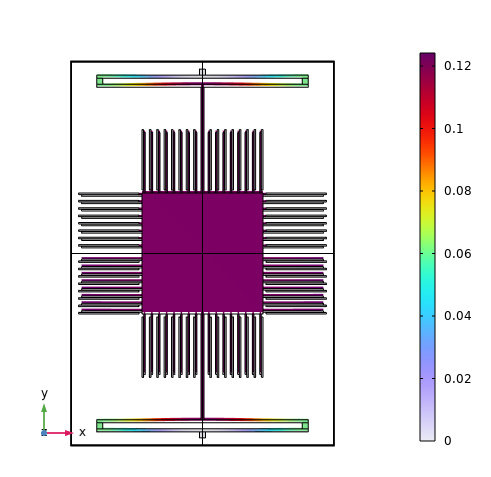
\includegraphics[width=1.0\linewidth]{displacement_ay}
        \caption{Displacement (\(\mu m\)) for acceleration \(a_y=50g\).}
        \label{fig:disp_ay}
    \end{figure}
    
    \begin{figure}[!h]
        \centering
        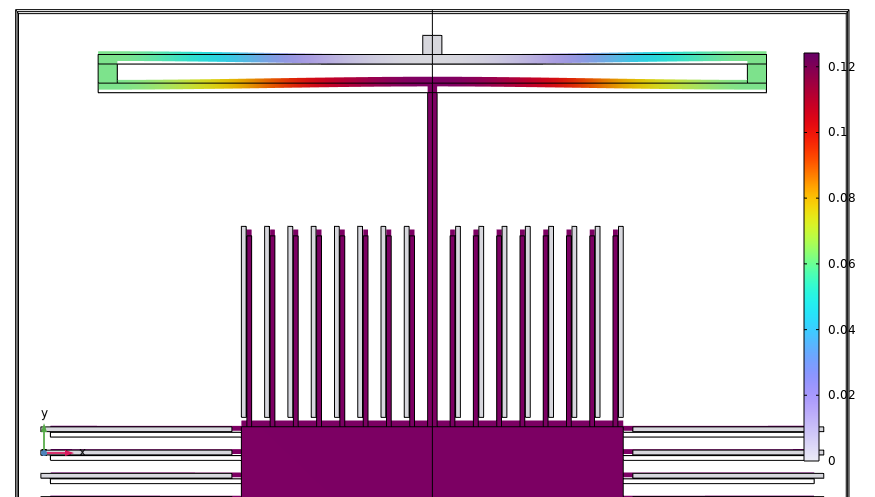
\includegraphics[width=1.0\linewidth]{displacement_ay_detail}
        \caption{Displacement (\(\mu m\)) for acceleration \(a_y=50g\), detail.}
        \label{fig:disp_ay_det}
    \end{figure}
    
    The maximum von Mises stress simulated for \(a_y=50g\) is \(2.6339\cdot10^6Pa\), which is almost identical to what is obtained in \cite{original} (\(2.5348\cdot10^6Pa\)). The same conclusions as before apply.
    
    \begin{figure}[!h]
        \centering
        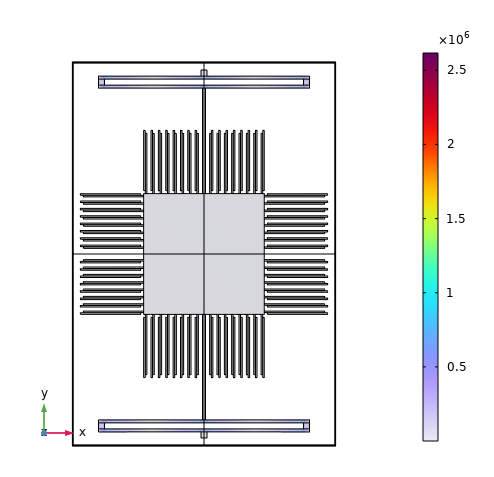
\includegraphics[width=1.0\linewidth]{stress_ay}
        \caption{Von Mises stress intensity (\(N/m^2\)) for acceleration \(a_y=50g\).}
        \label{fig:stress_ay}
    \end{figure}
    
    \begin{figure}[!h]
        \centering
        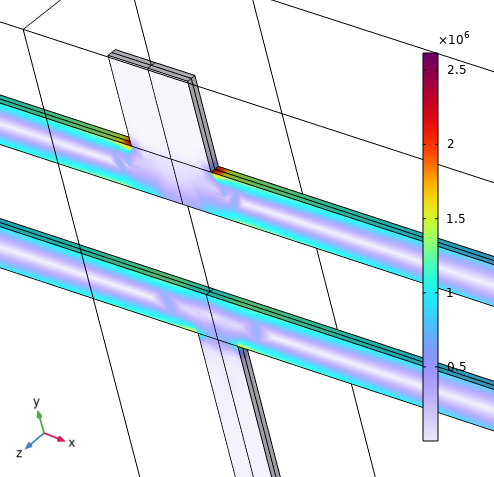
\includegraphics[width=1.0\linewidth]{stress_ay_detail}
        \caption{Von Mises stress intensity (\(N/m^2\)) for acceleration \(a_y=50g\), detail of the folded beam attachment to the anchor.}
        \label{fig:stress_ay_det}
    \end{figure}
    
    \bigskip
    \subsubsection{\(t_{bx}\) parametric sweep}
    
    \bigskip
    \subsubsection{\(w_{bx}\) parametric sweep}
        
    
    \section{Conclusions}
    
    \printbibliography
\end{document}